% IEEE Access-style manuscript.
% NOTE: the official ieeeaccess.cls was not available when this was prepared, so the local
% approximation ieeeaccessapprox.cls is used. For submission, move the body into the official
% IEEE Access template (https://ieeeaccess.ieee.org/) and use \documentclass{ieeeaccess}.
\documentclass{ieeeaccessapprox}
\usepackage{amsmath,amssymb}
\usepackage{graphicx}
\usepackage{booktabs}
\usepackage{multirow}
\usepackage{url}
\usepackage{enumitem}
\usepackage{cite}
\usepackage{dblfloatfix}
\usepackage[hidelinks,pdfusetitle]{hyperref}
\newcommand{\nParams}{1{,}055{,}081}
\newcommand{\nMACsG}{2.53}
\newcommand{\nSpatial}{883{,}472}
\newcommand{\nTemporal}{37{,}968}
\newcommand{\nFusion}{132{,}480}
\newcommand{\nHeads}{1{,}161}
\newcommand{\pSpatial}{83.7}
\newcommand{\pTemporal}{3.6}
\newcommand{\pFusion}{12.6}
\newcommand{\pBlockOne}{54}
\newcommand{\pBlocksOneTwo}{82}
\newcommand{\nWithin}{149}
\newcommand{\nTrials}{150}
\newcommand{\nMainsDb}{22}
\newcommand{\ampBefore}{0.152}
\newcommand{\ampAfter}{0.0125}
\newcommand{\noiseRef}{0.0212}
\newcommand{\notchLo}{49.18}
\newcommand{\notchHi}{50.83}
\newcommand{\notchW}{1.65}
\newcommand{\notchDb}{97}
\newcommand{\oneHzDb}{5.8}
\newcommand{\gdTen}{6.1}
\newcommand{\gdTwenty}{3.1}
\newcommand{\gdThirty}{2.8}
\newcommand{\covTotal}{95.1}
\newcommand{\nStmts}{548}
\newcommand{\nHit}{521}
\newcommand{\covTrain}{75.3}
\newcommand{\nFullMods}{8}
\newcommand{\nMods}{12}
\newcommand{\atrophyROI}{40}
\newcommand{\lesionROI}{180}
\newcommand{\retLesion}{99.7}
\newcommand{\retAtrophy}{0}

\newcommand{\accFull}{78.1}
\newcommand{\sdFull}{2.3}
\newcommand{\nFull}{7}
\newcommand{\accMRI}{68.0}
\newcommand{\accVEP}{64.0}
\newcommand{\accCat}{77.5}
\newcommand{\accSum}{79.6}
\newcommand{\gainUni}{10.7}
\newcommand{\gainUniP}{<0.001}
\newcommand{\nGainUni}{5}
\newcommand{\dCat}{+0.7}
\newcommand{\pCat}{=0.629}
\newcommand{\dSum}{-1.4}
\newcommand{\pSum}{=0.465}
\newcommand{\ablMin}{-1.7}
\newcommand{\ablMax}{+0.0}
\newcommand{\ablSig}{0}
\newcommand{\ablN}{7}
\newcommand{\sdAll}{4.3}
\newcommand{\accVone}{77.2}
\newcommand{\sdVone}{7.0}
\newcommand{\nSeedsMax}{7}

\newcommand{\todo}[1]{\colorbox{yellow}{[#1]}}
\newcommand{\cafn}{CAFN}
\def\UrlBreaks{\do\/\do\-\do\_\do\.\do\=}
\setlist[itemize]{leftmargin=1.2em,itemsep=1pt,topsep=2pt,parsep=0pt}
\setlist[enumerate]{leftmargin=1.5em,itemsep=1pt,topsep=2pt,parsep=0pt}

\history{Date of publication xxxx 00, 0000, date of current version xxxx 00, 0000.}
\doi{10.1109/ACCESS.2026.DOI}

\title{Cross-Attention Fusion of 3D MRI and 1D Electrophysiology for Vision-Pathway Disorders: A Controlled Benchmark and a Reproducible Multi-Cohort Evaluation}

\author{\uppercase{Mishthi Jain}\authorrefmark{1}}
\address[1]{School of Computer Science and Engineering, Vellore Institute of Technology, Chennai, India (e-mail: \todo{author e-mail})}
\tfootnote{This work was carried out as a BCSE497J project at the School of Computer Science and Engineering, Vellore Institute of Technology, Chennai. \todo{funding statement, if any}}
\markboth{M. Jain: Cross-Attention Fusion of 3D MRI and 1D Electrophysiology}{M. Jain: Cross-Attention Fusion of 3D MRI and 1D Electrophysiology}
\corresp{Corresponding author: Mishthi Jain (e-mail: \todo{author e-mail}).}

\begin{document}
\maketitle

\begin{abstract}
Disorders of the visual pathway alter both anatomy, visible on structural MRI, and signal timing, recorded as the visual evoked potential (VEP), yet most computational tools use only one of the two, and no public dataset pairs them with diagnosis labels. We present the Cross-Attention Fusion Network (CAFN), which couples a squeeze-and-excitation 3D residual encoder and a multi-scale 1D encoder through gated bidirectional cross-attention, and evaluate it in two ways. In a controlled synthetic benchmark in which the class information carried by each modality is tunable, fusion improved test accuracy by \gainUni{} percentage points over the better single modality ($\accFull\%$ versus $\accMRI\%$ and $\accVEP\%$), but cross-attention was statistically indistinguishable from concatenation ($\accCat\%$) and element-wise sum ($\accSum\%$), and none of seven component ablations produced a reliable change. On two public OpenNeuro cohorts (95 subjects; depression with MEG and zoster neuralgia with sleep EEG, each with T1-weighted MRI), evaluated with pooled and leave-one-cohort-out protocols, repeated cross-validation and permutation tests, neural fusion was at chance (AUC 0.51), a weak spectral signal was detectable (AUC 0.56--0.62), and nothing transferred between cohorts. The one-command pipeline runs from download to test statistics under a fixed seed and is supported by a 340-test suite. We report where fusion helps, where it does not, and the pitfalls we found; no diagnostic accuracy is claimed.
\end{abstract}

\begin{keywords}
Cross-attention, deep learning, explainability, glaucoma, magnetic resonance imaging, multimodal fusion, optic neuritis, visual evoked potentials.
\end{keywords}

\titlepgskip=-15pt

\section{Introduction}
\PARstart{V}{ision} depends on an uninterrupted chain of structures: the retina, the optic nerve, the optic chiasm, the lateral geniculate nucleus, the optic radiations and the visual cortex. A lesion anywhere along the chain can degrade sight, and the clinical picture depends on where the damage lies and on whether it disturbs the anatomy, the conduction of the electrical signal, or both. Glaucoma, a progressive optic neuropathy, had an estimated global prevalence of 3.54\% among people aged 40 to 80 years, or about 64.3 million people in 2013 \cite{tham2014}, and its degeneration extends to the intracranial optic nerve, the lateral geniculate nucleus and the visual cortex \cite{gupta2006}. Optic neuritis is characterised electrophysiologically by a delayed P100 peak of the visual evoked potential (VEP) \cite{halliday1972}, and cortical visual impairment (CVI) arises from damage to the brain's visual pathways \cite{sakki2018}.

Two investigations are routinely used to examine this pathway, and they answer different questions. Structural MRI gives a three-dimensional picture of anatomy, so that atrophy and focal lesions can be localised, but it carries no timing information. The VEP is a one-dimensional recording whose latency and amplitude, in particular those of the P100 component, reflect conduction in the pathway \cite{odom2016}, but it carries no spatial localisation. Combining complementary modalities has long been proposed as a way to reveal relationships that no single modality shows \cite{calhoun2016}.

Learning such a combination faces four obstacles. Most pipelines analyse only one modality (\emph{unimodal isolation}). A volume and a waveform differ in dimensionality, sampling and noise, and simple fusion by concatenation gives every feature the same standing (\emph{cross-modal heterogeneity}). A black-box classifier is difficult to trust clinically (\emph{limited interpretability}). Finally, no public dataset offers paired MRI, VEP and diagnosis labels (\emph{the labelling gap}). Published multimodal fusion studies with cross-attention \cite{zhou2024camf,dhar2025drifa} also tend to report a single headline number, which makes it hard to tell \emph{when} fusion is responsible for a gain.

This paper presents the Cross-Attention Fusion Network (CAFN) and, more importantly, an evaluation designed to answer that question honestly in a setting where real paired data are scarce. The contributions are:
\begin{enumerate}
\item \textbf{Architecture.} CAFN couples a squeeze-and-excitation 3D residual encoder and a multi-scale 1D encoder through \emph{gated bidirectional} cross-attention (each stream queries the other), with learned attention pooling, positional embeddings and two auxiliary unimodal heads. All pooling is implemented with deterministic matrix products, so GPU training is reproducible.
\item \textbf{A controlled benchmark of when fusion helps.} A synthetic generator with independent knobs for the class information carried by each modality allows a like-for-like comparison of cross-attention against concatenation, element-wise sum and unimodal models, a component ablation of seven design choices, and a sweep over modality informativeness, all with multiple seeds and a held-out test set.
\item \textbf{A reproducible real-data protocol.} A one-command pipeline downloads two public OpenNeuro cohorts (major depressive disorder with MEG, zoster-associated neuralgia with sleep EEG, each with T1-weighted MRI), preprocesses them, and evaluates pooled and leave-one-cohort-out models with repeated cross-validation, bootstrap intervals, label-permutation tests and classical baselines, under a single fixed random seed.
\item \textbf{Candid findings.} We report where the proposed design helps, where it does not, and that on the available real cohorts the signal is at most weak and does not transfer between cohorts, together with the pitfalls we found (Section~\ref{sec:discussion}).
\end{enumerate}
The code is available at \url{https://github.com/Mishthijainn/NeuroImaging}. Section~\ref{sec:related} reviews related work, Section~\ref{sec:method} describes the framework, Section~\ref{sec:setup} the experimental protocol, Section~\ref{sec:results} the results, and Sections~\ref{sec:discussion} and~\ref{sec:conclusion} discuss and conclude.

\section{Related Work}\label{sec:related}
\subsection{Deep learning for volumetric neuroimaging}
Three-dimensional CNNs are the standard tool for volumetric scans: multi-scale 3D CNNs were developed for brain-lesion segmentation \cite{kamnitsas2017}, and the 3D U-Net showed dense volumetric segmentation from sparse annotation \cite{cicek2016}. Residual connections \cite{he2016} carry over to 3D, and squeeze-and-excitation (SE) blocks re-weight channels from global context \cite{hu2018}; both are used in our spatial encoder. Brain extraction is a prerequisite for many pipelines, with dedicated tools such as HD-BET \cite{isensee2019} and SynthStrip \cite{hoopes2022}; MONAI provides the resampling transforms we use \cite{cardoso2022}.

\subsection{Evoked-potential conditioning and 1D CNNs}
Evoked potentials are conditioned to remove drift, muscle noise and mains interference. A Butterworth filter has a maximally flat pass-band \cite{butterworth1930} and a narrow IIR notch removes the mains frequency; applying a filter forward and backward cancels its phase \cite{gustafsson1996,oppenheim2010}, which matters because clinical VEP interpretation rests on latency \cite{odom2016}.

\subsection{Multimodal fusion and cross-attention}
Surveys distinguish early, intermediate and late fusion \cite{baltrusaitis2019,ramachandram2017}. Scaled dot-product attention lets queries select among keys and values \cite{vaswani2017}, vision transformers treat images as token sequences \cite{dosovitskiy2021}, and cross-modal attention relates modalities that are not aligned \cite{tsai2019,lu2019}. In neuroimaging, CAMF fuses structural and functional MRI for schizophrenia with self- and cross-attention and reports that cross-attention with adaptive weights beats concatenation and element-wise sum \cite{zhou2024camf}; DRIFA-Net applies dual attention with iterative alignment to five public medical-imaging datasets \cite{dhar2025drifa}. Table~\ref{tab:lit} summarises what these studies used and reported. To our knowledge no published study fuses MRI with an electrophysiological signal for visual-pathway disorders, and no public dataset with paired MRI, VEP and these diagnoses exists.

\begin{table*}[!t]
\caption{Published cross-attention fusion studies versus this work. Numbers are those reported by the authors on \emph{their} data; they are \textbf{not} comparable with ours (different tasks, modalities and data).}
\label{tab:lit}
\centering\footnotesize
\begin{tabular}{@{}p{0.13\textwidth}p{0.15\textwidth}p{0.21\textwidth}p{0.14\textwidth}p{0.26\textwidth}@{}}
\toprule
Study & Modalities & Data (size) & Task & Reported result\\
\midrule
CAMF \cite{zhou2024camf} & sMRI + fMRI (both 3D imaging) & COBRE+FBIRN+MPRC (620 subjects); BSNIP (442) as independent test & Schizophrenia vs control & Acc.\ 74.4\%, F1 0.705, MCC 0.491 (BSNIP: 67.9\%, 0.684, 0.361); cross-attention $>$ concat., sum, single modality\\
DRIFA-Net \cite{dhar2025drifa} & Dermoscopy, cytology, CT, MRI slices; BraTS MRI & HAM10000 (10{,}015), SIPaKMeD (4{,}049), brain-tumour MRI (7{,}023), IQ-OTHNCCD (1{,}098), BraTS2020 (369) & 3--7-class classification; segmentation & Acc.\ 95.6--99.7\% (D1--D4); both attention modules $>$ either alone\\
\textbf{This work} & 3D T1w MRI + 1D electrophysiology (heterogeneous) & Controlled synthetic benchmark; two OpenNeuro cohorts (95 subjects) & Control vs patient; 3-class synthetic & See Section~\ref{sec:results}\\
\bottomrule
\end{tabular}
\end{table*}

\subsection{Explainability}
Grad-CAM uses class-score gradients with respect to convolutional activations to localise evidence \cite{selvaraju2017}. Attention weights are not automatically faithful explanations \cite{jain2019,wiegreffe2019}, and saliency maps can be insensitive to model parameters \cite{adebayo2018}; our explainability outputs are therefore inspection aids, and we do not evaluate their faithfulness here.

\subsection{Public data and the labelling gap}
Public resources exist for structural and functional neuroimaging and electrophysiology \cite{vanessen2013,benson2018,lamontagne2019,gramfort2013,goldberger2000}, but none provides Healthy/Glaucoma/Optic-Neuritis-CVI labels with paired MRI and VEP. We therefore (i) study the architecture on controlled synthetic data and (ii) test the whole pipeline on the closest public data we could find that pairs a T1-weighted MRI with a resting electrophysiological recording and has patient and control groups \cite{liuzzi2022ds003568,ds007181}.

\section{The CAFN Framework}\label{sec:method}
\subsection{Overview}
CAFN takes a paired sample of a 3D MRI volume and a 1D signal and predicts a class. Figure~\ref{fig:pipeline} shows the data flow. A single configuration module fixes shapes and hyper-parameters so that preprocessing, both encoders, the fusion module and the training loop cannot disagree. The default configuration has $d_{\mathrm{model}}=128$, four heads, 64 spatial and 16 temporal tokens and 1.95\,M trainable parameters.

\begin{figure*}[!t]
\centering
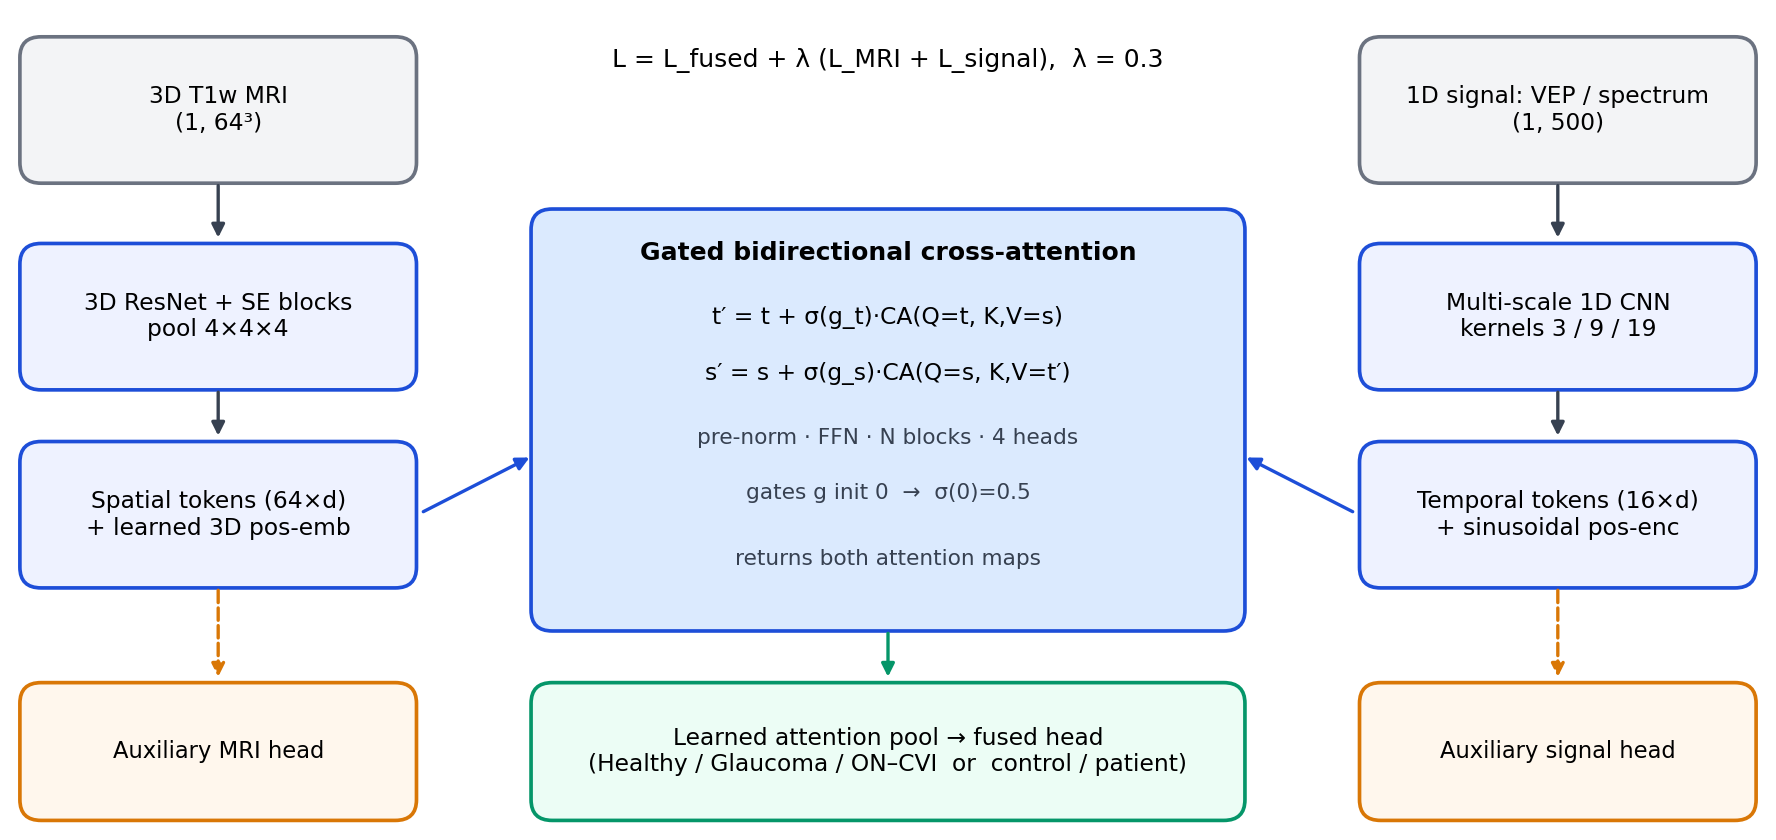
\includegraphics[width=0.66\textwidth]{figs/fig_arch_v2.png}
\caption{Data flow of CAFN. Preprocessed MRI and signal streams are encoded into spatial and temporal tokens, exchanged through gated bidirectional cross-attention, pooled by a learned attention pool and classified; two auxiliary heads read the unimodal tokens.}
\label{fig:pipeline}
\end{figure*}

\subsection{Preprocessing}\label{sec:mri}
\emph{MRI.} Volumes are reoriented to RAS, resampled to 1\,mm isotropic spacing and masked. Two foreground masks are implemented: an intensity-percentile mask (the original lightweight stand-in) and an Otsu threshold with hole filling and largest-component clean-up. For real whole-head T1w scans the volume is cropped to the foreground bounding box, resampled to $64^3$ (or $32^3$ for the cross-validation study), and normalised by a foreground z-score. A centre crop to $64^3$, which suffices for the small synthetic volumes, would see only a sliver of a 170\,mm head. Neither mask is a substitute for validated skull-stripping \cite{isensee2019,hoopes2022}.

\emph{VEP.} Records are validated, band-passed (4th-order Butterworth, 1--100\,Hz), notched at 50\,Hz ($Q=30$), both applied forward and backward so that the effective response is zero-phase,
\begin{equation}
H_{\mathrm{zp}}(\omega)=\lvert H(j\omega)\rvert^{2},\qquad \arg H_{\mathrm{zp}}(\omega)=0,
\end{equation}
resampled to 500 samples and z-scored. P100 latency is therefore not shifted.

\emph{Spectrum mode (real cohorts).} The public cohorts contain resting MEG or EEG, not VEPs. Each recording is reduced to the channel-averaged $\log_{10}$ Welch power spectral density between 1 and 45\,Hz, interpolated to 500 points and z-scored; the temporal encoder then operates on the spectrum and no time-domain filtering is applied.

\subsection{Encoders}
The spatial encoder is a stem (Conv3d, batch norm, ReLU) followed by three residual blocks (16$\to$32$\to$64$\to$128 channels, stride 2), each with a squeeze-and-excitation gate (reduction 4) \cite{hu2018}, and an adaptive average pool to $4\times4\times4$ giving $X_s\in\mathbb{R}^{64\times d}$ plus a learned 3D positional embedding. The temporal encoder is a stem followed by three strided stages, each followed by a \emph{multi-scale residual} block of parallel convolutions with kernels 3, 9 and 19, so that both a narrow peak and a broad waveform complex are visible; an adaptive pool gives 16 tokens $X_t\in\mathbb{R}^{16\times d}$ plus a sinusoidal positional encoding. All adaptive pooling is implemented as a per-axis matrix product with the exact PyTorch window weights; this is numerically equal to \texttt{AdaptiveAvgPool} but deterministic on CUDA and supported on Apple MPS.

\subsection{Gated bidirectional cross-attention}
In the original design only spatial tokens queried temporal tokens. CAFN now updates \emph{both} streams in each of $N$ pre-norm blocks, temporal first so that the spatial read consumes the enriched temporal tokens:
\begin{align}
t' &= t + \sigma(g_t)\,\mathrm{CA}\big(\mathrm{LN}(t),\,s\big),\quad t'\leftarrow t'+\mathrm{FFN}_t(\mathrm{LN}(t')),\\
s' &= s + \sigma(g_s)\,\mathrm{CA}\big(\mathrm{LN}(s),\,t'\big),\quad s'\leftarrow s'+\mathrm{FFN}_s(\mathrm{LN}(s')),
\end{align}
where $\mathrm{CA}(q,kv)$ is multi-head scaled dot-product attention with queries from $q$ and keys and values from $kv$,
\begin{equation}
\mathrm{CA}=\mathrm{softmax}\!\Big(\frac{QK^{\top}}{\sqrt{d_h}}\Big)V,\qquad d_h=d/H,
\end{equation}
and $g_s,g_t$ are learned scalar gates initialised at zero ($\sigma(0)=0.5$: both directions start half open). The fused spatial tokens are layer-normalised and pooled with a learned attention pool whose near-zero initial scorer reproduces mean pooling at the start of training.

\subsection{Objective and baselines}
Three linear heads read the pooled fused tokens, the mean spatial tokens and the mean temporal tokens. With cross-entropy losses $L_f,L_s,L_t$, $L=L_f+\lambda(L_s+L_t)$ with $\lambda=0.3$; class weights (inverse frequency) and label smoothing are optional. For like-for-like comparison we implement the fusion strategies used in the literature \cite{zhou2024camf}: \emph{concatenation} (mean-pooled streams concatenated and projected), \emph{element-wise sum}, and the two unimodal references (\emph{MRI only}, \emph{VEP/spectrum only}); all share the encoders, the auxiliary loss and the training recipe. The original one-way fusion with mean pooling and no positional encoding or SE is the \emph{v1-style} configuration.

\subsection{Explainability}
3D Grad-CAM (and Grad-CAM++) is computed on the last residual block from the fused logit, and the attention tensors of both directions are returned for plotting per head. A P100 latency estimator with an ISCEV-aligned search window converts the VEP stream into a clinician-checkable number. These are inspection aids, not clinical evidence.

\subsection{Controlled synthetic generator}\label{sec:synth}
A seeded generator produces class-conditioned MRI volumes (an ellipsoidal brain with ventricles; Glaucoma: a focal hypointensity, Optic Neuritis/CVI: a focal hyperintensity at a random location) and VEP records (N75--P100--N145 complex with class-specific latency and amplitude drawn per subject: $100\pm3$\,ms/$6.0\pm0.8$, $104\pm4$\,ms/$2.5\pm0.6$ and $138\pm6$\,ms/$4.0\pm1.0$ for the three classes, plus drift, mains and muscle noise). Two parameters, $\mu_{\mathrm{MRI}},\mu_{\mathrm{VEP}}\in[0,1]$, scale how far the lesion contrast and the VEP latency and amplitude offsets move from the healthy class (1: default generator; 0: no class signal). Because the two modalities are generated independently given the label, their evidence is complementary by construction; this is the setting in which fusion \emph{should} help, and the study asks how reliably each architecture exploits it.

\section{Experimental Setup}\label{sec:setup}
\subsection{Implementation and reproducibility}
CAFN is implemented in PyTorch \cite{paszke2019} with MONAI \cite{cardoso2022}, NiBabel, MNE-Python \cite{gramfort2013}, SciPy \cite{virtanen2020} and scikit-learn. All randomness derives from one constant seed (42; repeat $k$ uses $42{+}k$), deterministic algorithms are requested, and a single script (\texttt{run\_all.sh}) performs download, preprocessing, training, validation and testing and records the environment. Neural models were trained on an NVIDIA RTX 3050 Laptop GPU (4\,GB) with mixed precision; the model needs under 1\,GB at batch size 8. To finish in time, some synthetic runs were distributed over an Apple M3 Max (CPU or MPS) and the host CPU; every run is reproducible on its own device at a fixed seed, but results are not bit-identical across devices; all configurations of a given seed ran on the same device, so the paired comparisons between configurations are not affected.

\subsection{Study A: controlled synthetic benchmark}
Each (setting, seed) draws 144 training, 48 validation and 120 test samples (test drawn from a different seed range), $32^3$ MRI volumes and 500-point VEPs; checkpoints are selected on validation balanced accuracy and \emph{all} reported numbers are on the test set. The main setting ($\mu_{\mathrm{MRI}}=1.0$, $\mu_{\mathrm{VEP}}=0.3$) was fixed from a pilot that trained only the two unimodal models and chose the difficulty at which both were clearly above chance and below saturation; it was not tuned on CAFN. Twelve configurations (Table~\ref{tab:ablation}) are run on at least five seeds (more for the five key comparisons). A sweep varies $\mu_{\mathrm{VEP}}$ (MRI fixed) for four methods.

\subsection{Study B: real cohorts}
Two public OpenNeuro datasets with a patient group, a control group, a T1-weighted MRI and a resting recording are used (Table~\ref{tab:cohorts}): ds003568 (major depressive disorder vs healthy adolescents, MEG) \cite{liuzzi2022ds003568} and ds007181 (zoster-associated neuralgia vs healthy controls, whole-night polysomnographic EEG) \cite{ds007181}. Only subjects with both a T1w scan and a usable recording are kept (95 of 117 listed). The label is pan-disorder (0 control, 1 patient), which is a deliberate and important limitation.

\begin{table}[!t]
\caption{Real cohorts used (subjects with both modalities).}
\label{tab:cohorts}
\centering\scriptsize\setlength{\tabcolsep}{3pt}
\begin{tabular}{@{}lllrr@{}}
\toprule
Cohort & Patients vs controls & Signal & Ctrl & Pat\\
\midrule
ds003568 & MDD vs healthy & resting MEG (CTF) & 18 & 29\\
ds007181 & Zoster neuralgia vs healthy & PSG EEG & 27 & 21\\
\bottomrule
\end{tabular}
\end{table}

\emph{Protocols.} (i) \emph{Cohort split}: each cohort is split 70/15/15 (train/val/test); a pooled model is reported per cohort, and \emph{leave-one-cohort-out} (LODO) trains on one cohort and tests on every subject of the other. (ii) \emph{Repeated cross-validation}: every subject is predicted out-of-fold in 5-fold CV stratified on cohort and label, repeated five times for classical models and once for the neural models, so metrics use all 95 subjects instead of the 7-subject test splits. Classical baselines are logistic regression on the 500-point spectrum, on five band powers (delta 1--4, theta 4--8, alpha 8--13, beta 13--30, gamma 30--45\,Hz) and on PCA-reduced MRI ($8^3$ voxels $\to$ 20 components), a random forest on band powers, and MRI plus band powers. Neural variants (CAFN, concatenation, MRI only, spectrum only) use a regularised configuration ($d_{\mathrm{model}}=64$, dropout 0.3, weight decay $10^{-2}$) fixed in advance. (iii) \emph{Statistics}: ROC-AUC and balanced accuracy, a 1000-resample bootstrap 95\% interval over subjects, and a 200-permutation test that shuffles labels \emph{within} each cohort (preserving cohort base rates, so a cohort-identity shortcut cannot produce significance).

\subsection{Metrics}
Accuracy, macro-F1 and balanced accuracy for the three-class synthetic task; ROC-AUC and balanced accuracy for the binary real task. Differences between methods on the synthetic study are paired over seeds.

\section{Results}\label{sec:results}
\subsection{Study A: when does fusion help? (synthetic benchmark)}\label{sec:studyA}
Table~\ref{tab:ablation} and Fig.~\ref{fig:ablation} compare twelve configurations at the preset difficulty ($\mu_{\mathrm{MRI}}{=}1.0$, $\mu_{\mathrm{VEP}}{=}0.3$; chance is 33.3\%). Two results are clear and one is not.

\emph{Fusion helps, a lot.} The two unimodal references reach only 68.0\% (MRI only, $n{=}5$ seeds) and 64.0\% (VEP only, $n{=}4$), whereas every fusion model is at 77.5--79.6\%. The full CAFN improves on the better unimodal model (MRI only) by 10.7 percentage points (paired over 5 seeds, SD 2.7, paired $t$-test $p<0.001$). This confirms the premise of multimodal fusion in the setting where the evidence in the two modalities is complementary.

\emph{The specific fusion mechanism does not matter at this scale.} CAFN (78.1$\pm$2.3\%, $n{=}7$) is statistically indistinguishable from concatenation (77.5$\pm$2.3\%; paired difference +0.7$\pm$3.3, $p=0.629$) and from element-wise sum (79.6$\pm$3.4\%; -1.4$\pm$4.3, $p=0.465$). Removing any single design choice (bidirectionality, positional encoding, attention pooling, SE blocks, the auxiliary loss, or adding a second fusion block) changes the mean accuracy by between -1.7 and +0.0 points, whose magnitude is smaller than the seed-to-seed standard deviation (about 4.3 points); 0 of 7 of these differences is nominally significant ($p<0.05$, uncorrected). The v1-style configuration with everything switched off scores 77.2\% ($\Delta=-1.5$, $p=0.629$), but with a much larger spread (7.0 versus 2.3 points), which is in line with the training instability we observed earlier for the v1 recipe. We therefore make \emph{no} claim that gated bidirectional cross-attention improves accuracy over simpler fusion on this benchmark.

\begin{table}[!t]
\caption{Study A (synthetic, three classes, $\mu_{\mathrm{MRI}}{=}1.0$, $\mu_{\mathrm{VEP}}{=}0.3$): test performance of the fused head (mean $\pm$ SD over seeds). $\Delta$: mean paired difference in accuracy to the full CAFN, in percentage points.}
\label{tab:ablation}
\centering\scriptsize\setlength{\tabcolsep}{2.5pt}
\begin{tabular}{@{}lcccc@{}}
\toprule
Configuration & Params (M) & Acc.\ (\%) & Macro-F1 (\%) & $\Delta$\\
\midrule
CAFN (full) & 1.96 & $78.1\pm2.3$ & $78.0\pm2.4$ & -- \\
w/o bidirectional & 1.82 & $77.0\pm5.5$ & $76.7\pm5.1$ & -1.7 \\
w/o positional enc. & 1.95 & $78.7\pm3.9$ & $78.5\pm3.9$ & -0.0 \\
w/o attention pooling & 1.96 & $77.7\pm2.1$ & $77.2\pm2.2$ & -1.0 \\
w/o SE blocks & 1.94 & $77.5\pm5.9$ & $76.8\pm6.8$ & -1.2 \\
w/o auxiliary loss & 1.96 & $77.3\pm5.7$ & $77.2\pm5.8$ & -1.3 \\
2 fusion blocks & 2.22 & $77.0\pm1.6$ & $76.5\pm2.1$ & -1.7 \\
v1-style (all off) & 1.80 & $77.2\pm7.0$ & $76.7\pm7.1$ & -1.5 \\
Concatenation & 1.72 & $77.5\pm2.3$ & $77.1\pm2.4$ & -0.7 \\
Element-wise sum & 1.69 & $79.6\pm3.4$ & $79.4\pm3.3$ & +1.4 \\
MRI only & 1.69 & $68.0\pm4.7$ & $66.0\pm5.9$ & -10.7 \\
VEP only & 1.69 & $64.0\pm4.3$ & $63.5\pm4.4$ & -14.6 \\

\bottomrule
\end{tabular}
\end{table}

\begin{figure}[!t]
\centering
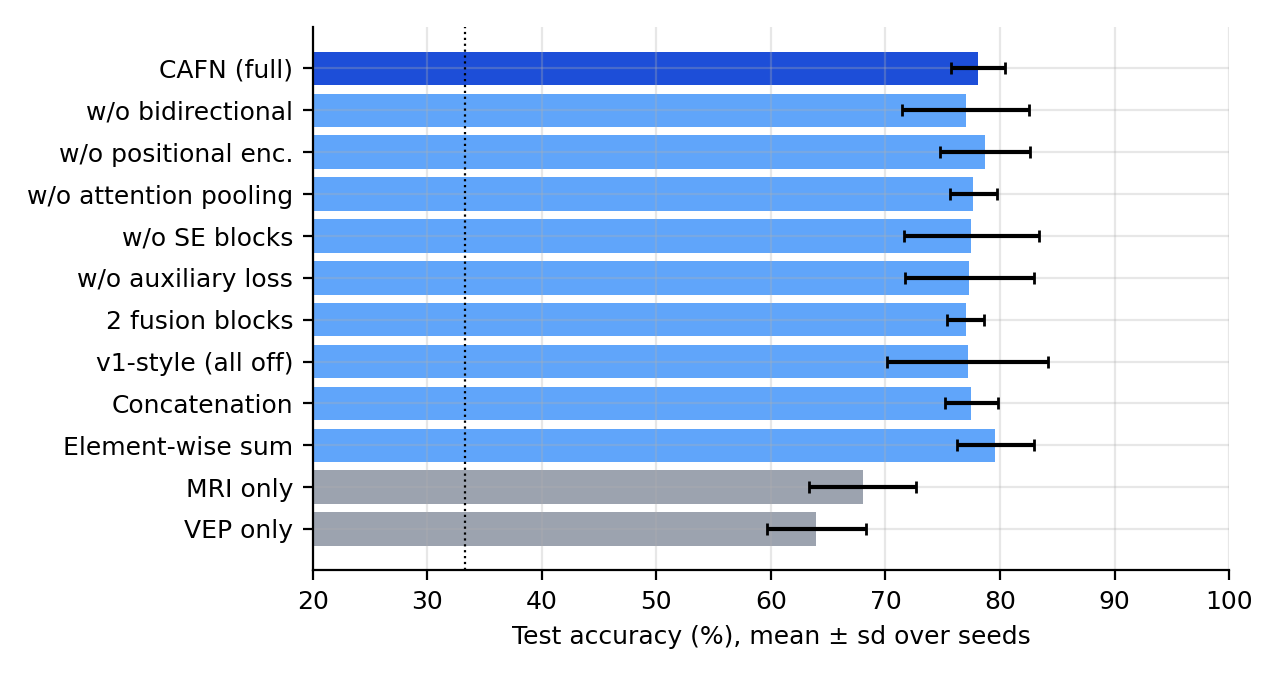
\includegraphics[width=\columnwidth]{figs/fig_ablation.png}
\caption{Study A: test accuracy by configuration (bars: mean, whiskers: SD over seeds; dotted line: chance). Grey: unimodal references.}
\label{fig:ablation}
\end{figure}

\subsection{Study A: how informative must each modality be?}
Fig.~\ref{fig:sweep} varies $\mu_{\mathrm{VEP}}$ with the MRI fixed ($n{=}2$ seeds per point; four methods). The VEP-only model rises from chance (45\%) to 97\% while the MRI-only model stays at 63--70\%. The gain of the fused models over the better single modality is largest at intermediate informativeness and vanishes when one modality dominates: +5 points (CAFN) and +7 (concatenation) at $\mu_{\mathrm{VEP}}{=}0.15$, +13 points (CAFN) and +12 (concatenation) at $\mu_{\mathrm{VEP}}{=}0.3$, +5 points (CAFN) and +5 (concatenation) at $\mu_{\mathrm{VEP}}{=}0.5$, +1 points (CAFN) and +2 (concatenation) at $\mu_{\mathrm{VEP}}{=}1$. Fusion therefore never hurt here, helps when both streams carry independent evidence, and converges to the dominant stream otherwise; CAFN and concatenation track each other throughout. With only 2 seeds per point the intervals are wide and the curves should be read as a trend, not as precise estimates.

\begin{figure}[!t]
\centering
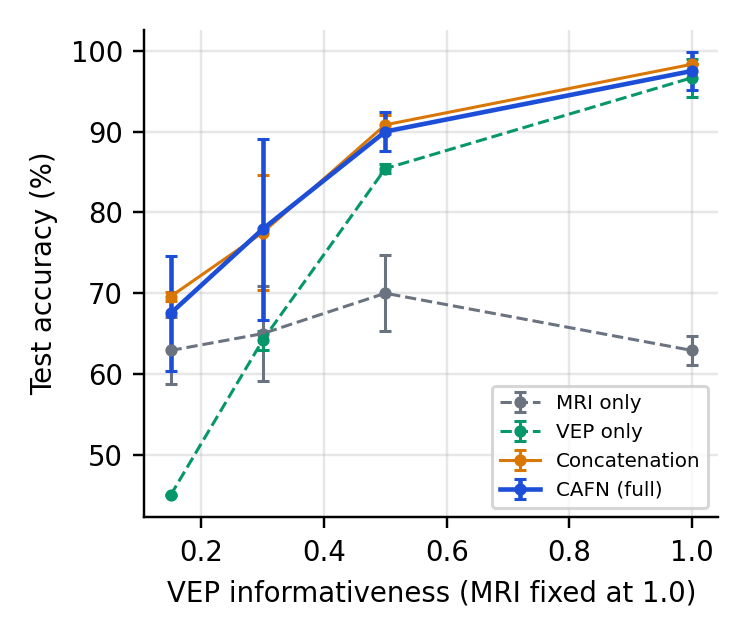
\includegraphics[width=0.78\columnwidth]{figs/fig_sweep.png}
\caption{Study A sweep: test accuracy versus VEP informativeness (MRI fixed at 1.0). Dashed: unimodal models; solid: fusion models.}
\label{fig:sweep}
\end{figure}

\subsection{Real cohorts: cross-validated classification}\label{sec:realcv}
Table~\ref{tab:realcv} and Fig.~\ref{fig:realcv} report out-of-fold performance for all 95 subjects (50 patients, 45 controls). \emph{The signal is weak and fragile.} Linear models on spectral features reach an AUC of 0.56--0.57 (balanced accuracy 0.59). The within-cohort permutation test gives $p=0.005$ for the five band powers and $p=0.025$ for the full spectrum, which is nominally significant but, with five classical models tested, only the band-power model survives a Bonferroni correction ($p_{\mathrm{adj}}=0.025$); its bootstrap interval ([0.45, 0.68]) still includes 0.5, so the evidence is at best suggestive. A random forest on the same features is at chance ($p=0.73$), and MRI-derived features (PCA of an $8^3$ down-sampled volume) are not distinguishable from chance either ($p=0.24$). The neural models tell the same story: the best is the \emph{spectrum-only} network (AUC 0.62, interval [0.50, 0.72]); the full CAFN (0.51), concatenation (0.53) and MRI-only (0.48) networks are at chance. Adding the MRI stream therefore did \emph{not} help on these cohorts; if anything it hurt, consistent with an MRI branch that overfits 76 training subjects per fold.

\begin{table}[!t]
\caption{Real cohorts (95 subjects): out-of-fold ROC-AUC (mean over repeats; classical models 5 repeats of 5-fold CV, neural models 1 repeat), bootstrap 95\% CI (repeat~0), balanced accuracy and within-cohort permutation $p$ (200 permutations).}
\label{tab:realcv}
\centering\scriptsize\setlength{\tabcolsep}{2.5pt}
\begin{tabular}{@{}lcccc@{}}
\toprule
Model & AUC & 95\% CI & Bal.\ acc. & Perm.\ $p$\\
\midrule
Spectrum (500-pt) $\cdot$ LogReg & $0.563$ & [0.45, 0.68] & $0.590$ & 0.025 \\
Band powers (5) $\cdot$ LogReg & $0.567$ & [0.45, 0.68] & $0.590$ & 0.005 \\
Band powers (5) $\cdot$ Random forest & $0.518$ & [0.36, 0.60] & $0.539$ & 0.726 \\
MRI (8$^3$ $\rightarrow$ PCA-20) $\cdot$ LogReg & $0.587$ & [0.43, 0.67] & $0.584$ & 0.239 \\
MRI + band powers $\cdot$ LogReg & $0.588$ & [0.43, 0.67] & $0.580$ & 0.234 \\
CAFN (ours) & $0.510$ & [0.40, 0.62] & $0.518$ & -- \\
Concatenation fusion & $0.533$ & [0.42, 0.66] & $0.553$ & -- \\
MRI only & $0.479$ & [0.36, 0.60] & $0.503$ & -- \\
Spectrum only & $0.618$ & [0.50, 0.72] & $0.561$ & -- \\

\bottomrule
\end{tabular}
\end{table}

\begin{figure}[!t]
\centering
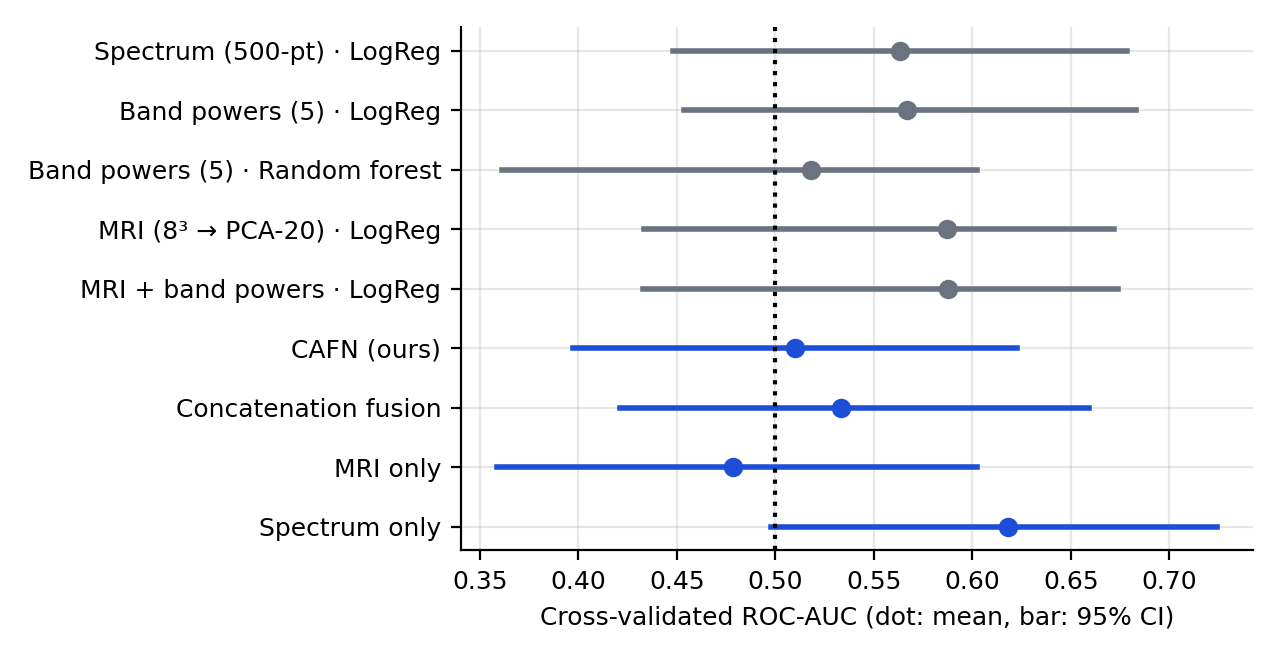
\includegraphics[width=\columnwidth]{figs/fig_real_cv.png}
\caption{Cross-validated AUC on the real cohorts (dot: mean, bar: 95\% bootstrap CI). Grey: classical models; blue: neural models. The dotted line is chance.}
\label{fig:realcv}
\end{figure}

\subsection{Cohort split and leave-one-cohort-out}\label{sec:lodo}
Table~\ref{tab:cohortcafn} shows the full CAFN ($64^3$ MRI) trained on the pooled cohorts and evaluated on each cohort's held-out test subjects (7 per cohort), and trained on one cohort and tested on every subject of the other. All accuracies lie between 0.45 and 0.52 and balanced accuracies between 0.46 and 0.54: at chance, with variation across repeats larger than any difference between settings. Fig.~\ref{fig:realcurves} shows why: the training loss falls to nearly zero within 30 epochs while validation accuracy stays near 0.5, i.e.\ the model memorises the roughly 67 training subjects. The classical models do not transfer either (Table~\ref{tab:lodo}): across cohorts the AUC ranges from 0.40 to 0.63 and the balanced accuracy is 0.43--0.51; the spectrum model's AUC of 0.63 when trained on ds007181 and tested on ds003568 comes with a balanced accuracy of 0.50, showing that the ranking transfers weakly while the decision threshold does not (different sensors and recording protocols shift the spectrum). A linear model identifies the cohort from the spectrum alone with 100\% accuracy, so cohort identity is an available shortcut; the within-cohort permutation test in Section~\ref{sec:realcv} is designed not to reward it.

\begin{table}[!t]
\caption{CAFN on the real cohorts (mean $\pm$ SD over 3 repeats; test subjects only).}
\label{tab:cohortcafn}
\centering\scriptsize\setlength{\tabcolsep}{2.5pt}
\begin{tabular}{@{}lccc@{}}
\toprule
Setting & Accuracy & Bal.\ acc. & AUC\\
\midrule
Pooled, test (both cohorts, $n{=}14$) & $0.52\pm0.04$ & $0.52\pm0.04$ & $0.61\pm0.09$ \\
Pooled, test ds003568 ($n{=}7$) & $0.52\pm0.08$ & $0.46\pm0.07$ & $0.61\pm0.17$ \\
Pooled, test ds007181 ($n{=}7$) & $0.52\pm0.08$ & $0.54\pm0.07$ & $0.53\pm0.17$ \\
Leave ds003568 out ($n{=}47$) & $0.48\pm0.09$ & $0.46\pm0.04$ & $0.57\pm0.08$ \\
Leave ds007181 out ($n{=}48$) & $0.45\pm0.02$ & $0.49\pm0.05$ & $0.44\pm0.03$ \\

\bottomrule
\end{tabular}
\end{table}

\begin{table}[!t]
\caption{Leave-one-cohort-out for classical models: AUC / balanced accuracy when tested on the named cohort after training on the other.}
\label{tab:lodo}
\centering\scriptsize\setlength{\tabcolsep}{2.5pt}
\begin{tabular}{@{}lcc@{}}
\toprule
Model & ds003568 & ds007181\\
\midrule
Spectrum (500-pt) $\cdot$ LogReg & 0.63 / 0.50 & 0.57 / 0.50 \\
Band powers (5) $\cdot$ LogReg & 0.50 / 0.50 & 0.48 / 0.50 \\
Band powers (5) $\cdot$ Random forest & 0.50 / 0.50 & 0.50 / 0.50 \\
MRI (8$^3$ $\rightarrow$ PCA-20) $\cdot$ LogReg & 0.40 / 0.43 & 0.44 / 0.47 \\
MRI + band powers $\cdot$ LogReg & 0.41 / 0.43 & 0.46 / 0.51 \\

\bottomrule
\end{tabular}
\end{table}

\begin{figure}[!t]
\centering
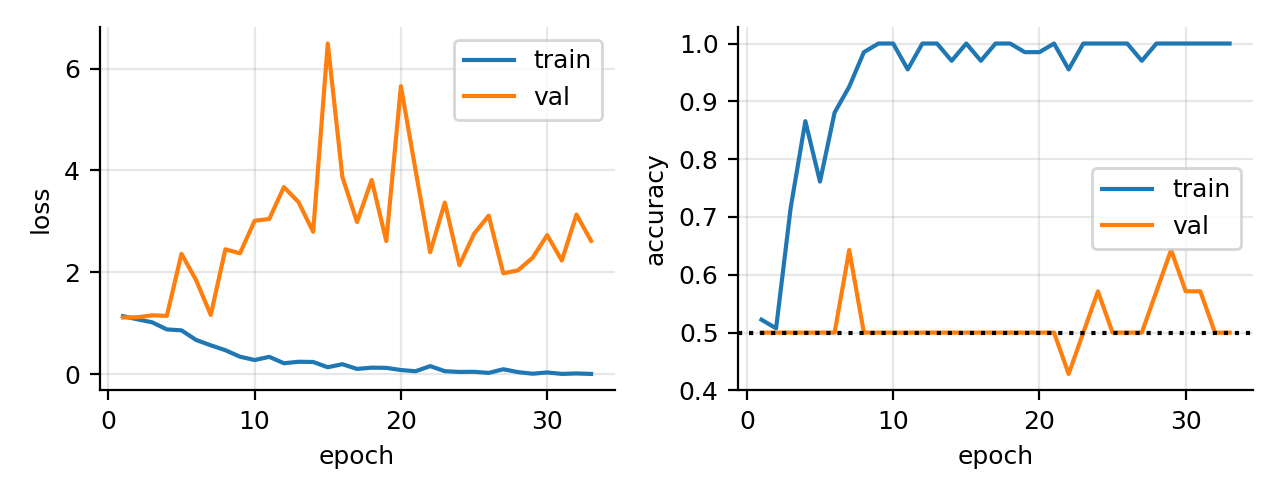
\includegraphics[width=\columnwidth]{figs/fig_real_curves.png}
\caption{Pooled CAFN, repeat 0: training versus validation loss and accuracy on the real cohorts. The validation curve stays near chance while the training loss vanishes.}
\label{fig:realcurves}
\end{figure}

\subsection{Signal conditioning on synthetic VEPs}
The VEP conditioning chain was verified on 150 seeded synthetic records (50 per class; 250\,Hz). The 50\,Hz response of the forward--backward notch is $-\notchDb$\,dB, the fitted 50\,Hz amplitude fell from \ampBefore{} to \ampAfter{} (mean reduction \nMainsDb\,dB, a lower bound set by the noise floor), and the P100 latency was recovered within one sample (4\,ms) in \nWithin{} of \nTrials{} records (Table~\ref{tab:p100}). A single-pass implementation of the same filters, with a group delay of \gdTen, \gdTwenty{} and \gdThirty\,ms at 10, 20 and 30\,Hz, was indistinguishable at this sampling rate, so the case for zero-phase processing rests on the principle that latency is the clinical quantity \cite{odom2016}, not on an empirical gain.

\begin{figure}[!t]
\centering
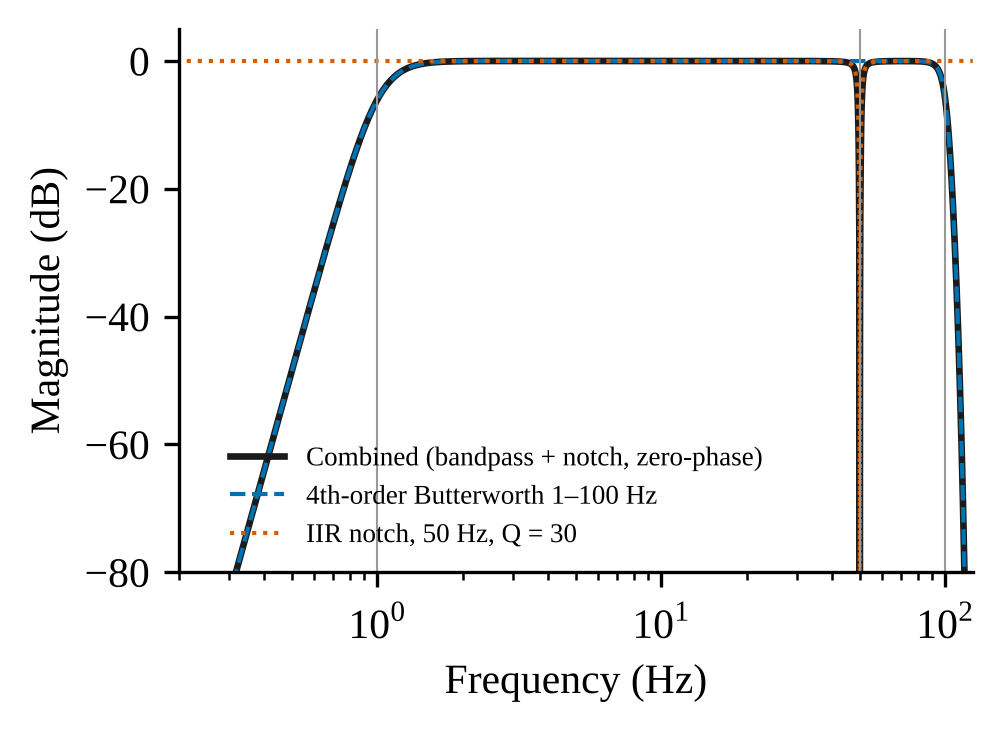
\includegraphics[width=\columnwidth]{figs/fig_filter_col.png}
\caption{Effective (forward--backward) magnitude response of the conditioning filters.}
\label{fig:filter}
\end{figure}

\begin{table}[!t]
\caption{Detected P100 latency in ms (mean $\pm$ SD over 50 synthetic trials per class).}
\label{tab:p100}
\centering\footnotesize
\begin{tabular}{@{}lcccc@{}}
\toprule
Class & True & Raw & Zero-phase & Single-pass\\
\midrule
Healthy Control & 100 & $101.8\pm2.3$ & $100.6\pm1.9$ & $101.1\pm1.8$ \\
Glaucoma & 108 & $107.4\pm2.7$ & $108.0\pm2.9$ & $108.2\pm2.3$ \\
Optic Neuritis/CVI & 140 & $141.3\pm2.5$ & $140.8\pm2.1$ & $141.0\pm2.7$
\\
\bottomrule
\end{tabular}
\end{table}

\subsection{Model size, cost and software verification}
The default three-class CAFN has \textbf{1{,}955{,}140} trainable parameters and 2.60\,G multiply--accumulates per sample at $64^3$ (0.39\,G at $32^3$) (Table~\ref{tab:params}); the 3D spatial encoder holds 46\% of the parameters and 97\% of the compute, the multi-scale temporal encoder 40\% of the parameters, and the gated bidirectional fusion 14\% of the parameters but under 0.5\% of the compute. The repository's automated suite now contains 340 tests (unit and integration, including end-to-end runs of the command-line tools, the cohort loaders and the experiment runner); all pass on macOS with Python 3.14, and on Ubuntu 22.04 with Python 3.12 and CUDA (one test is skipped on that host). Running on a second platform exposed three latent defects that the first platform had masked (a type annotation that fails on Python $\le$3.13, a device mismatch in the evaluation-only path on CUDA, and a unit test whose assertion was mathematically vacuous); all were fixed. The two real-file readers (CTF MEG and EDF polysomnography) were checked on real recordings, and the deterministic adaptive pooling was verified to match PyTorch's pooling in forward and backward passes.

\begin{table}[!t]
\caption{Trainable parameters and multiply--accumulates (M, at $64^3$) per component of the default CAFN.}
\label{tab:params}
\centering\footnotesize
\begin{tabular}{@{}lrr@{}}
\toprule
Component & Parameters & MACs (M)\\
\midrule
Spatial encoder (3D ResNet + SE) & 894{,}504 & 2522.68 \\
Temporal encoder (multi-scale 1D CNN) & 785{,}936 & 65.89 \\
Gated bidirectional fusion & 265{,}218 & 11.01 \\
Positional embeddings & 8{,}192 & 0.00 \\
Attention pool & 129 & 0.00 \\
Heads (3) & 1{,}161 & 0.00 \\
\midrule
Total & 1{,}955{,}140 & 2600 \\

\bottomrule
\end{tabular}
\end{table}

\section{Discussion}\label{sec:discussion}
\subsection{What the evidence supports}
\emph{(1) Fusion helps when both modalities carry independent evidence.} In the controlled benchmark every fusion model beat the better single modality by about \gainUni{} points (CAFN, $n{=}\nGainUni$ paired seeds, $p\gainUniP$), and the sweep shows that this advantage is largest at intermediate informativeness and disappears when one modality dominates. This is the behaviour the multimodal-fusion literature assumes \cite{calhoun2016,baltrusaitis2019}, now measured under controlled conditions.

\emph{(2) The fusion mechanism mattered little.} Gated bidirectional cross-attention was statistically indistinguishable from concatenation (\dCat{} points, $p\pCat$) and element-wise sum (\dSum{}, $p\pSum$), and none of the seven single-component ablations produced a reliable change (range \ablMin{} to \ablMax{} points; $\ablSig$ of $\ablN$ nominally significant). CAMF reports that cross-attention beats concatenation and summation by roughly 1--3 accuracy points (arXiv version) on real schizophrenia data \cite{zhou2024camf}, a gap of the order of our seed-to-seed standard deviation (\sdAll{} points); we can neither confirm nor refute it, but at this model and sample size we do not find that the extra machinery buys accuracy. What cross-attention does provide is a by-product that concatenation lacks: attention maps in both directions (and a P100 estimator) that can be inspected, which is the stated clinical motivation. The faithfulness of those maps is not established here.

\emph{(3) On the real cohorts the signal is weak, and fusion did not help.} Only the spectral stream carried a signal (AUC 0.56--0.62, with the neural spectrum-only model highest), the MRI stream was at chance, the fused models were at chance, and nothing transferred between cohorts. We regard this as the expected outcome rather than a failure of the pipeline: 95 subjects, two unrelated disorders pooled under one label, different sensors, and a model of about 2\,M parameters that memorises its $\sim$67 training subjects (Fig.~\ref{fig:realcurves}).

\subsection{Why the real-data result is null}
Several factors are confounded and cannot be separated with these data. (i)~\emph{Sample size}: 95 subjects give AUC intervals about $\pm0.12$ wide. (ii)~\emph{Label heterogeneity}: depression and zoster neuralgia are different conditions, so a single ``patient'' class is not one concept. (iii)~\emph{Surrogate signal}: the resting spectrum is not a VEP and no timing biomarker such as P100 latency is available. (iv)~\emph{Preprocessing}: skull-stripping is still a threshold mask. In a single-seed diagnostic on the synthetic generator, switching the MRI pipeline from a percentile mask with min--max scaling to an Otsu mask with foreground z-scoring dropped the MRI-only accuracy from 73\% to 41\%, so real-MRI preprocessing is a first-order variable. (v)~\emph{Cohort effects}: the spectrum identifies the cohort perfectly, so any pooled model can exploit site; the within-cohort permutation test and leave-one-cohort-out evaluation exist to expose that.

\subsection{Pitfalls we hit and fixed}
These are of independent practical interest: restoring the checkpoint with the lowest \emph{validation loss} restored an untrained epoch-1 model on short runs (the early validation loss spikes while batch-norm statistics settle), which is why selection is now on validation balanced accuracy; a centre crop of a whole-head scan to $64^3$ sees only a sliver of the head, which is why the real-MRI path crops to the foreground bounding box; PyTorch's adaptive average pooling has a non-deterministic CUDA backward and no Apple MPS kernel, which we replaced with an equivalent matrix-product implementation; and running on a second platform exposed three defects hidden on the first (Section~\ref{sec:results}).

\subsection{Limitations}
(i)~Study A is synthetic: the modalities are independent given the label by construction, which favours fusion; real data may behave differently. (ii)~The number of seeds is small (at most \nSeedsMax{} per configuration, two per sweep point), so only large effects are detectable. (iii)~The real cohorts are not eye-disease data, the label is pan-disorder, and the 1-D stream is a spectrum, not a VEP; no claim about glaucoma, optic neuritis or CVI follows. (iv)~Skull-stripping and harmonisation across scanners and sensors are crude. (v)~Neural models on real data were cross-validated once and have no permutation test. (vi)~Explainability outputs were not validated against ground truth. (vii)~Hyper-parameters of the real-data study were fixed in advance rather than tuned, so a better-tuned model might do somewhat better; we chose not to tune on 95 subjects.

\subsection{Contribution in context}
Relative to \cite{zhou2024camf,dhar2025drifa}, which report fusion gains on benchmark data, the contribution here is methodological rather than a new state of the art: a fusion architecture for \emph{heterogeneous} 3D-image + 1-D-signal pairs, a controlled benchmark that isolates the effect of fusion from the effect of architecture, a reproducible one-command evaluation protocol with cross-cohort and permutation-based statistics, and an explicit account of what does and does not hold.

\section{Conclusion and Future Work}\label{sec:conclusion}
We presented CAFN, a gated bidirectional cross-attention network for paired 3D MRI and 1D electrophysiology, and evaluated it in two ways. In a controlled synthetic benchmark fusion improved accuracy by about \gainUni{} points over the better single modality, while the choice among cross-attention, concatenation and summation, and every individual design component, made no reliable difference ($\accFull\%$ for CAFN versus $\accCat\%$ and $\accSum\%$). On two public real cohorts (95 subjects, pan-disorder label, T1w MRI plus resting MEG/EEG) neural fusion was at chance, a weak spectral signal (AUC about 0.56--0.62) was detectable, and nothing generalised across cohorts. The whole pipeline, from download to test statistics, runs from one command with a fixed seed. The next step is data, not architecture: a labelled, paired MRI--VEP cohort with patient-level splits; pre-trained or self-supervised encoders and strong regularisation for small samples; harmonisation across sites; validated skull-stripping; and checks of the attention and Grad-CAM maps against clinician-marked regions or the known lesion masks of the synthetic generator.

\section*{Acknowledgment}
The author thanks \todo{guide name and designation} for guidance throughout this project.

\begin{thebibliography}{39}
\bibitem{tham2014}
Y.-C. Tham, X. Li, T. Y. Wong, H. A. Quigley, T. Aung, and C.-Y. Cheng, ``Global prevalence of glaucoma and projections of glaucoma burden through 2040: A systematic review and meta-analysis,'' \emph{Ophthalmology}, vol. 121, no. 11, pp. 2081--2090, 2014, doi: 10.1016/j.ophtha.2014.05.013.
\bibitem{gupta2006}
N. Gupta, L.-C. Ang, L. No\"{e}l de Tilly, L. Bidaisee, and Y. H. Y\"{u}cel, ``Human glaucoma and neural degeneration in intracranial optic nerve, lateral geniculate nucleus, and visual cortex,'' \emph{Brit. J. Ophthalmol.}, vol. 90, no. 6, pp. 674--678, 2006, doi: 10.1136/bjo.2005.086769.
\bibitem{halliday1972}
A. M. Halliday, W. I. McDonald, and J. Mushin, ``Delayed visual evoked response in optic neuritis,'' \emph{Lancet}, vol. 299, no. 7758, pp. 982--985, 1972, doi: 10.1016/S0140-6736(72)91155-5.
\bibitem{sakki2018}
H. E. A. Sakki, N. J. Dale, J. Sargent, T. Perez-Roche, and R. Bowman, ``Is there consensus in defining childhood cerebral visual impairment? A systematic review of terminology and definitions,'' \emph{Brit. J. Ophthalmol.}, vol. 102, no. 4, pp. 424--432, 2018, doi: 10.1136/bjophthalmol-2017-310694.
\bibitem{odom2016}
J. V. Odom \emph{et al.}, ``ISCEV standard for clinical visual evoked potentials: (2016 update),'' \emph{Documenta Ophthalmol.}, vol. 133, no. 1, pp. 1--9, 2016, doi: 10.1007/s10633-016-9553-y.
\bibitem{calhoun2016}
V. D. Calhoun and J. Sui, ``Multimodal fusion of brain imaging data: A key to finding the missing link(s) in complex mental illness,'' \emph{Biol. Psychiatry, Cogn. Neurosci. Neuroimaging}, vol. 1, no. 3, pp. 230--244, 2016, doi: 10.1016/j.bpsc.2015.12.005.
\bibitem{kamnitsas2017}
K. Kamnitsas \emph{et al.}, ``Efficient multi-scale 3D CNN with fully connected CRF for accurate brain lesion segmentation,'' \emph{Med. Image Anal.}, vol. 36, pp. 61--78, 2017, doi: 10.1016/j.media.2016.10.004.
\bibitem{cicek2016}
\"{O}. \c{C}i\c{c}ek, A. Abdulkadir, S. S. Lienkamp, T. Brox, and O. Ronneberger, ``3D U-Net: Learning dense volumetric segmentation from sparse annotation,'' in \emph{Proc. Med. Image Comput. Comput.-Assist. Intervent. (MICCAI)}, 2016, pp. 424--432, doi: 10.1007/978-3-319-46723-8\_49.
\bibitem{he2016}
K. He, X. Zhang, S. Ren, and J. Sun, ``Deep residual learning for image recognition,'' in \emph{Proc. IEEE Conf. Comput. Vis. Pattern Recognit. (CVPR)}, 2016, pp. 770--778, doi: 10.1109/CVPR.2016.90.
\bibitem{isensee2019}
F. Isensee \emph{et al.}, ``Automated brain extraction of multisequence MRI using artificial neural networks,'' \emph{Hum. Brain Mapp.}, vol. 40, no. 17, pp. 4952--4964, 2019, doi: 10.1002/hbm.24750.
\bibitem{hoopes2022}
A. Hoopes, J. S. Mora, A. V. Dalca, B. Fischl, and M. Hoffmann, ``SynthStrip: Skull-stripping for any brain image,'' \emph{NeuroImage}, vol. 260, Art. no. 119474, 2022, doi: 10.1016/j.neuroimage.2022.119474.
\bibitem{cardoso2022}
M. J. Cardoso \emph{et al.}, ``MONAI: An open-source framework for deep learning in healthcare,'' 2022, \emph{arXiv:2211.02701}.
\bibitem{butterworth1930}
S. Butterworth, ``On the theory of filter amplifiers,'' \emph{Exp. Wireless Wireless Eng.}, vol. 7, pp. 536--541, 1930.
\bibitem{gustafsson1996}
F. Gustafsson, ``Determining the initial states in forward-backward filtering,'' \emph{IEEE Trans. Signal Process.}, vol. 44, no. 4, pp. 988--992, 1996, doi: 10.1109/78.492552.
\bibitem{oppenheim2010}
A. V. Oppenheim and R. W. Schafer, \emph{Discrete-Time Signal Processing}, 3rd ed. Upper Saddle River, NJ, USA: Pearson, 2010.
\bibitem{baltrusaitis2019}
T. Baltru\v{s}aitis, C. Ahuja, and L.-P. Morency, ``Multimodal machine learning: A survey and taxonomy,'' \emph{IEEE Trans. Pattern Anal. Mach. Intell.}, vol. 41, no. 2, pp. 423--443, 2019, doi: 10.1109/TPAMI.2018.2798607.
\bibitem{ramachandram2017}
D. Ramachandram and G. W. Taylor, ``Deep multimodal learning: A survey on recent advances and trends,'' \emph{IEEE Signal Process. Mag.}, vol. 34, no. 6, pp. 96--108, 2017, doi: 10.1109/MSP.2017.2738401.
\bibitem{vaswani2017}
A. Vaswani \emph{et al.}, ``Attention is all you need,'' in \emph{Proc. Adv. Neural Inf. Process. Syst. (NeurIPS)}, vol. 30, 2017, pp. 5998--6008.
\bibitem{dosovitskiy2021}
A. Dosovitskiy \emph{et al.}, ``An image is worth 16\texttimes16 words: Transformers for image recognition at scale,'' in \emph{Proc. Int. Conf. Learn. Represent. (ICLR)}, 2021.
\bibitem{tsai2019}
Y.-H. H. Tsai, S. Bai, P. P. Liang, J. Z. Kolter, L.-P. Morency, and R. Salakhutdinov, ``Multimodal transformer for unaligned multimodal language sequences,'' in \emph{Proc. 57th Annu. Meeting Assoc. Comput. Linguistics}, 2019, pp. 6558--6569, doi: 10.18653/v1/P19-1656.
\bibitem{lu2019}
J. Lu, D. Batra, D. Parikh, and S. Lee, ``ViLBERT: Pretraining task-agnostic visiolinguistic representations for vision-and-language tasks,'' in \emph{Proc. Adv. Neural Inf. Process. Syst. (NeurIPS)}, vol. 32, 2019, pp. 13--23.
\bibitem{selvaraju2017}
R. R. Selvaraju, M. Cogswell, A. Das, R. Vedantam, D. Parikh, and D. Batra, ``Grad-CAM: Visual explanations from deep networks via gradient-based localization,'' in \emph{Proc. IEEE Int. Conf. Comput. Vis. (ICCV)}, 2017, pp. 618--626, doi: 10.1109/ICCV.2017.74.
\bibitem{jain2019}
S. Jain and B. C. Wallace, ``Attention is not explanation,'' in \emph{Proc. Conf. North Amer. Chapter Assoc. Comput. Linguistics: Human Lang. Technol. (NAACL-HLT)}, 2019, pp. 3543--3556, doi: 10.18653/v1/N19-1357.
\bibitem{wiegreffe2019}
S. Wiegreffe and Y. Pinter, ``Attention is not not explanation,'' in \emph{Proc. Conf. Empirical Methods Natural Lang. Process. 9th Int. Joint Conf. Natural Lang. Process. (EMNLP-IJCNLP)}, 2019, pp. 11--20, doi: 10.18653/v1/D19-1002.
\bibitem{adebayo2018}
J. Adebayo, J. Gilmer, M. Muelly, I. Goodfellow, M. Hardt, and B. Kim, ``Sanity checks for saliency maps,'' in \emph{Proc. Adv. Neural Inf. Process. Syst. (NeurIPS)}, vol. 31, 2018, pp. 9505--9515.
\bibitem{vanessen2013}
D. C. Van Essen, S. M. Smith, D. M. Barch, T. E. J. Behrens, E. Yacoub, and K. Ugurbil, ``The WU-Minn Human Connectome Project: An overview,'' \emph{NeuroImage}, vol. 80, pp. 62--79, 2013, doi: 10.1016/j.neuroimage.2013.05.041.
\bibitem{benson2018}
N. C. Benson \emph{et al.}, ``The Human Connectome Project 7 Tesla retinotopy dataset: Description and population receptive field analysis,'' \emph{J. Vis.}, vol. 18, no. 13, Art. no. 23, 2018, doi: 10.1167/18.13.23.
\bibitem{lamontagne2019}
P. J. LaMontagne \emph{et al.}, ``OASIS-3: Longitudinal neuroimaging, clinical, and cognitive dataset for normal aging and Alzheimer disease,'' \emph{medRxiv}, 2019, doi: 10.1101/2019.12.13.19014902.
\bibitem{gramfort2013}
A. Gramfort \emph{et al.}, ``MEG and EEG data analysis with MNE-Python,'' \emph{Front. Neurosci.}, vol. 7, Art. no. 267, 2013, doi: 10.3389/fnins.2013.00267.
\bibitem{goldberger2000}
A. L. Goldberger \emph{et al.}, ``PhysioBank, PhysioToolkit, and PhysioNet: Components of a new research resource for complex physiologic signals,'' \emph{Circulation}, vol. 101, no. 23, pp. e215--e220, 2000, doi: 10.1161/01.CIR.101.23.e215.
\bibitem{paszke2019}
A. Paszke \emph{et al.}, ``PyTorch: An imperative style, high-performance deep learning library,'' in \emph{Proc. Adv. Neural Inf. Process. Syst. (NeurIPS)}, vol. 32, 2019, pp. 8024--8035.
\bibitem{virtanen2020}
P. Virtanen \emph{et al.}, ``SciPy 1.0: Fundamental algorithms for scientific computing in Python,'' \emph{Nature Methods}, vol. 17, no. 3, pp. 261--272, 2020, doi: 10.1038/s41592-019-0686-2.
\bibitem{harris2020}
C. R. Harris \emph{et al.}, ``Array programming with NumPy,'' \emph{Nature}, vol. 585, no. 7825, pp. 357--362, 2020, doi: 10.1038/s41586-020-2649-2.
\bibitem{hunter2007}
J. D. Hunter, ``Matplotlib: A 2D graphics environment,'' \emph{Comput. Sci. Eng.}, vol. 9, no. 3, pp. 90--95, 2007, doi: 10.1109/MCSE.2007.55.
\bibitem{zhou2024camf}
Z. Zhou, A. Orlichenko, G. Qu, Z. Fu, V. D. Calhoun, Z. Ding, and Y.-P. Wang, ``An interpretable cross-attentive multi-modal MRI fusion framework for schizophrenia diagnosis,'' 2024, \emph{arXiv:2404.00144}.
\bibitem{dhar2025drifa}
J. Dhar, N. Zaidi, M. Haghighat, S. Roy, P. Goyal, A. Alavi, and V. Kumar, ``Multimodal fusion learning with dual attention for medical imaging,'' in \emph{Proc. IEEE/CVF Winter Conf. Appl. Comput. Vis. (WACV)}, 2025, pp. 4362--4371, doi: 10.1109/WACV61041.2025.00428.
\bibitem{hu2018}
J. Hu, L. Shen, and G. Sun, ``Squeeze-and-excitation networks,'' in \emph{Proc. IEEE Conf. Comput. Vis. Pattern Recognit. (CVPR)}, 2018, pp. 7132--7141, doi: 10.1109/CVPR.2018.00745.
\bibitem{liuzzi2022ds003568}
L. Liuzzi, K. Chang, H. Keren, C. Zheng, D. Saha, D. Nielson, and A. Stringaris, ``Mood induction in MDD and healthy adolescents,'' OpenNeuro dataset ds003568, v1.0.4, 2023, doi: 10.18112/openneuro.ds003568.v1.0.4 (see also L. Liuzzi \emph{et al.}, ``Electrophysiological correlates of mood and reward dynamics in human adolescents,'' \emph{bioRxiv}, 2021, doi: 10.1101/2021.03.04.433969).
\bibitem{ds007181}
L. Li, Q. Han, H. Bai, X. Zhang, Y. Liu, and C. He, ``Structural MRI, resting-state fMRI, and PSG/EEG dataset of zoster-associated neuralgia,'' OpenNeuro dataset ds007181, v1.0.1, 2026, doi: 10.18112/openneuro.ds007181.v1.0.1.
\end{thebibliography}


\begin{biography}{}{Mishthi Jain}
is a B.Tech.\ student in Computer Science and Engineering (Artificial Intelligence and Machine Learning) at the Vellore Institute of Technology, Chennai, India. \todo{short biography and research interests}
\end{biography}
\EOD
\end{document}
